%===============================
\clearpage
\newpage
\section{Tracking: David dataset} 
%===============================
								\begin{figure}[h!]
								\centering
								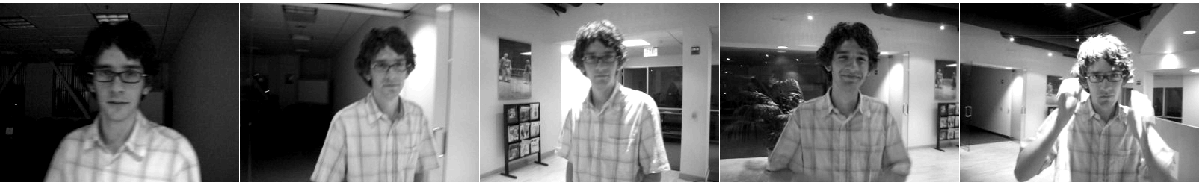
\includegraphics[width=1.0\textwidth]{figs/seq_2_davidin300.png}
								\caption{David dataset.}
								\label{fig:seq_1_David}
								\end{figure}



\begin{table}[h]
\centering
\begin{tabular}{|l|c|c|c|c|}
\hline
&\textbf{maxQ}&\textbf{RofE}&\textbf{nulE}&\textbf{monR}\\\hline
\textbf{2}&5.67&6.93&8.72&11.31\\\hline
\textbf{4}&4.39&5.95&4.59&5.00\\\hline
\textbf{8}&8.08&6.14&8.50&8.52\\\hline
\textbf{12}&6.07&5.65&6.70&4.52\\\hline
\textbf{16}&5.48&5.33&4.60&4.29\\\hline
\end{tabular}

\caption{Tracking errors for various RVQ configurations.  -1 means that track was lost.  These results show that RVQ is able to track the object of interest very closely.}
\end{table}

For the interested reader, detailed graphical results follow for 8x4 RVQ.

%------------------------------------
\clearpage
\newpage
\subsection{Tracking error}
%------------------------------------

								\begin{figure}[h!]
								\centering
								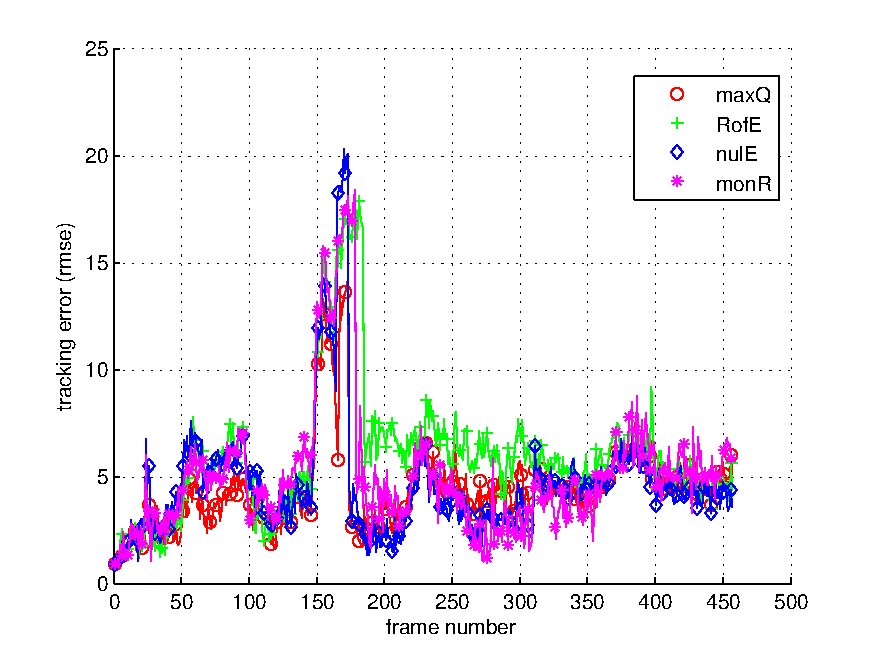
\includegraphics[height=0.38\textheight]{figs/2_davidin300_8_4_1000_trk_rmse.pdf}
								\caption{8x4 RVQ, tracking error (rmse).}
								\label{fig:2_davidin300_8_4_1000_trk_rmse}
								\end{figure}


								\begin{figure}[h!]
								\centering
								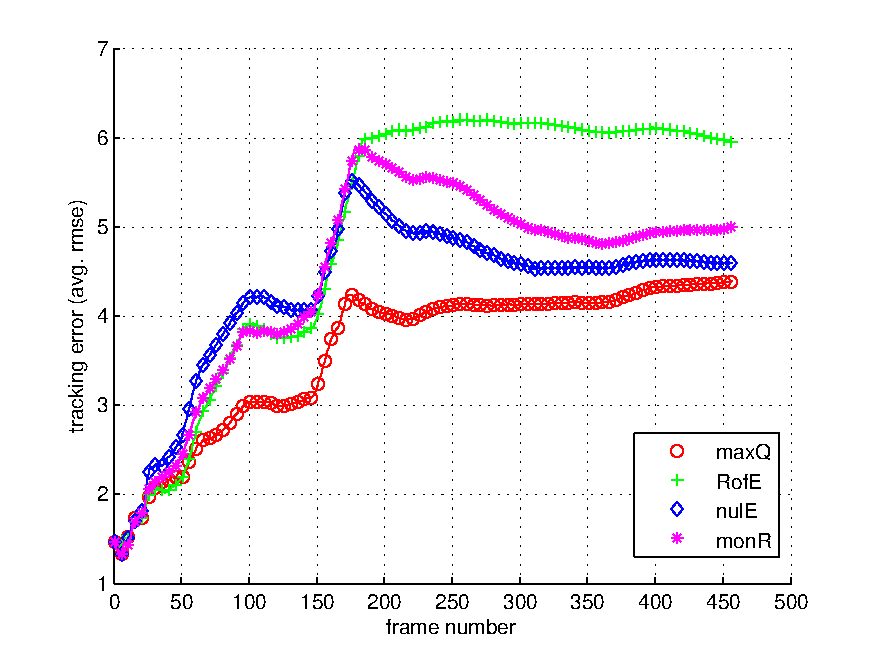
\includegraphics[height=0.38\textheight]{figs/2_davidin300_8_4_1000_trk_armse.pdf}
								\caption{8x4 RVQ, tracking error (average rmse).}
								\label{fig:2_davidin300_8_4_1000_trk_avg_rmse}
								\end{figure}

%------------------------------------
\clearpage
\newpage
\subsection{Target reconstruction}
%------------------------------------

								\begin{figure}[h!]
								\centering
								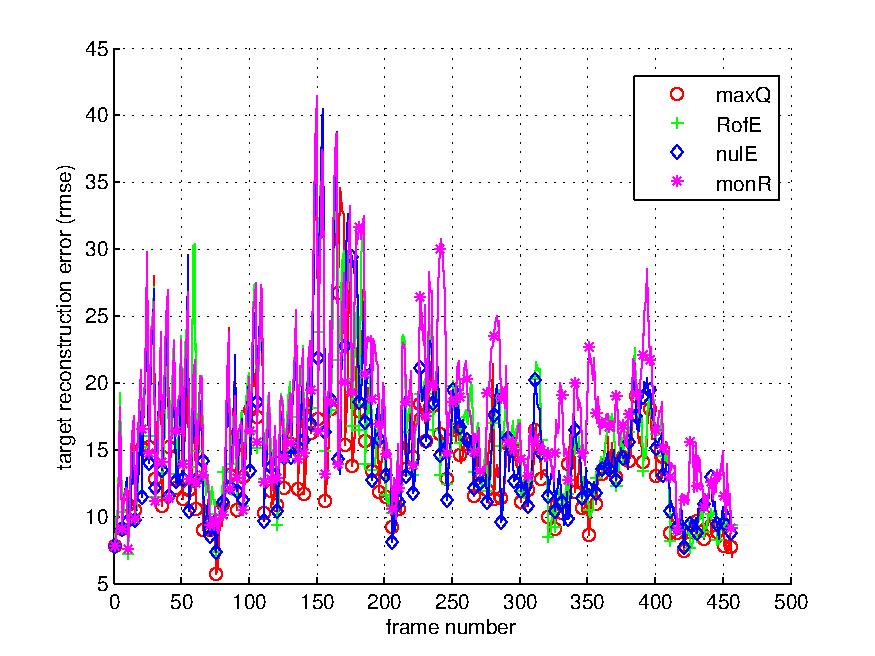
\includegraphics[height=0.4\textheight]{figs/2_davidin300_8_4_1000_snp_rmse.pdf}
								\caption{8x4 RVQ, snippet reconstruction error (rmse).}
								\label{fig:2_davidin300_8_4_1000_snp_rmse}
								\end{figure}


								\begin{figure}[h!]
								\centering
								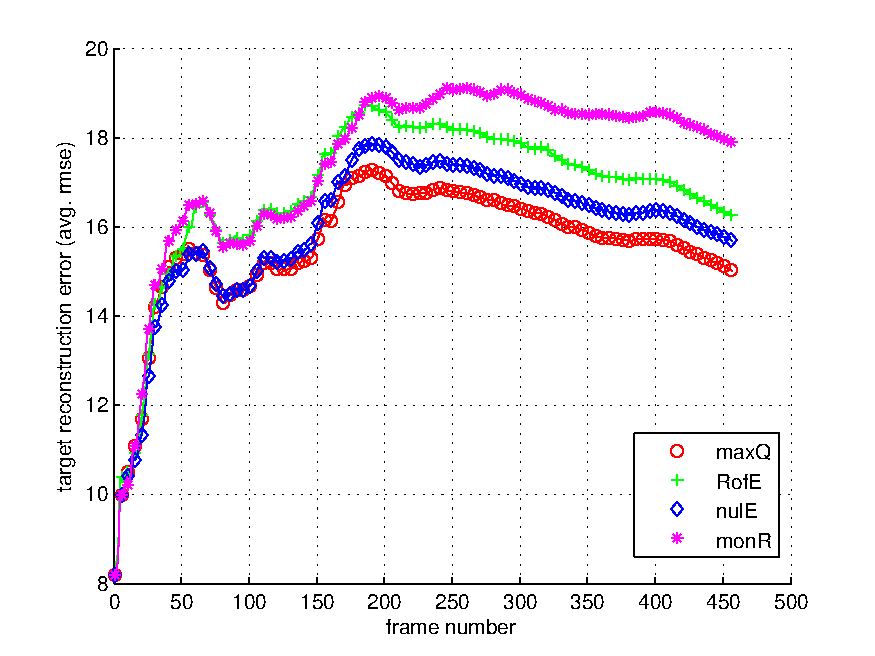
\includegraphics[height=0.4\textheight]{figs/2_davidin300_8_4_1000_snp_armse.pdf}
								\caption{8x4 RVQ, snippet reconstruction error (avg. rmse).}
								\label{fig:2_davidin300_8_4_1000_snp_armse}
								\end{figure}

								\begin{figure}[h!]
								\centering
								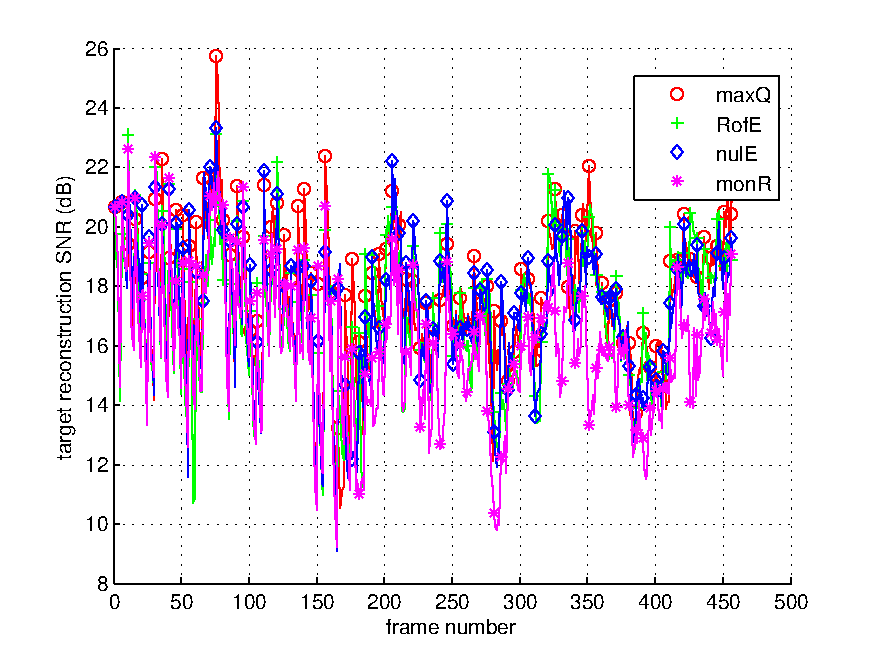
\includegraphics[height=0.4\textheight]{figs/2_davidin300_8_4_1000_snp_SNRdB.pdf}
								\caption{8x4 RVQ, snippet reconstruction SNR in dB.}
								\label{fig:2_davidin300_8_4_1000_snp_SNRdB}
								\end{figure}
%------------------------------------
\clearpage
\newpage
\subsection{Learning}
%------------------------------------

								\begin{figure}[h!]
								\centering
								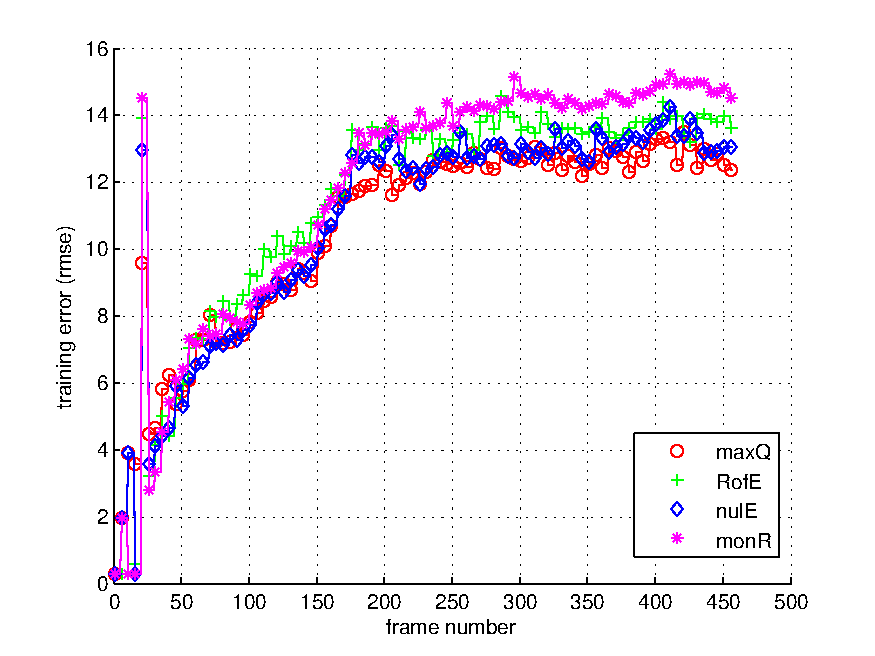
\includegraphics[height=0.4\textheight]{figs/2_davidin300_8_4_1000_trg_rmse.pdf}
								\caption{8x4 RVQ, training error (rmse).}
								\label{fig:2_davidin300_8_4_1000_trg_rmse}
								\end{figure}


								\begin{figure}[h!]
								\centering
								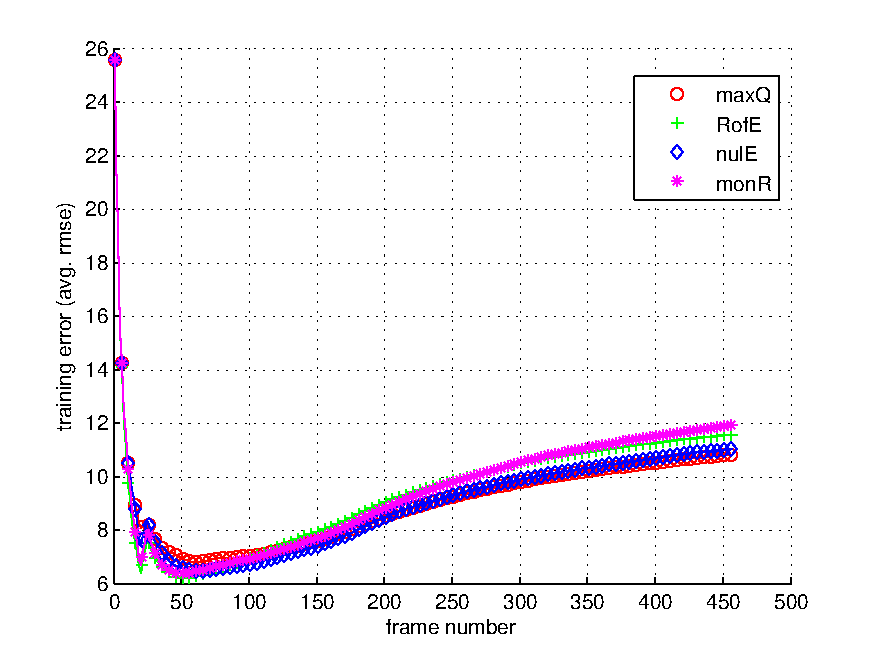
\includegraphics[height=0.4\textheight]{figs/2_davidin300_8_4_1000_trg_armse.pdf}
								\caption{8x4 RVQ, training error (avg. rmse).}
								\label{fig:2_davidin300_8_4_1000_trg_armse}
								\end{figure}

								\begin{figure}[h!]
								\centering
								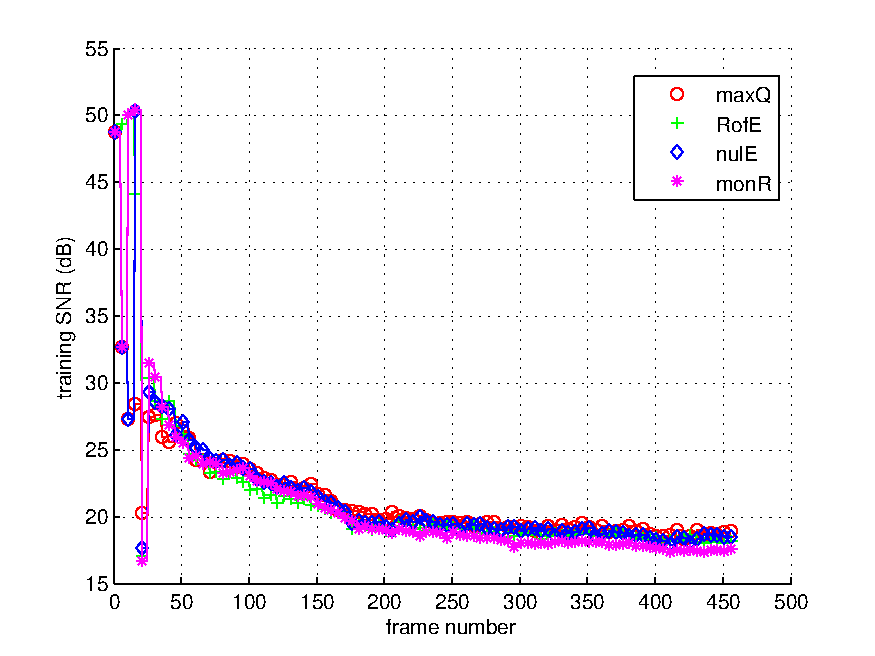
\includegraphics[height=0.4\textheight]{figs/2_davidin300_8_4_1000_trg_SNRdB.pdf}
								\caption{8x4 RVQ, training SNR in dB.}
								\label{fig:2_davidin300_8_4_1000_trg_SNRdB}
								\end{figure}
%------------------------------------
\clearpage
\newpage
\subsection{Testing}
%------------------------------------
								\begin{figure}[h!]
								\centering
								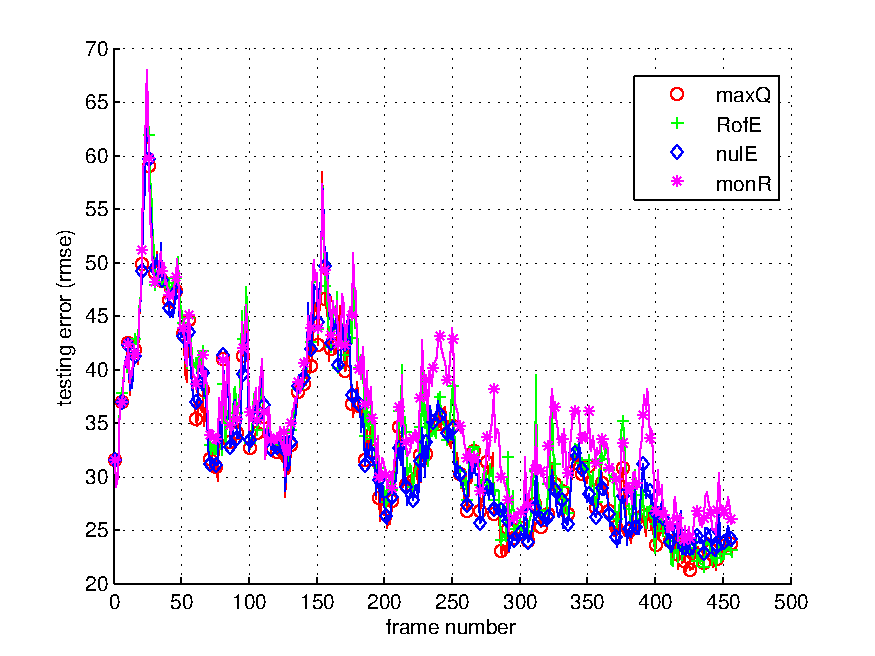
\includegraphics[height=0.4\textheight]{figs/2_davidin300_8_4_1000_tst_rmse.pdf}
								\caption{8x4 RVQ, testing error (rmse).}
								\label{fig:2_davidin300_8_4_1000_tst_rmse}
								\end{figure}


								\begin{figure}[h!]
								\centering
								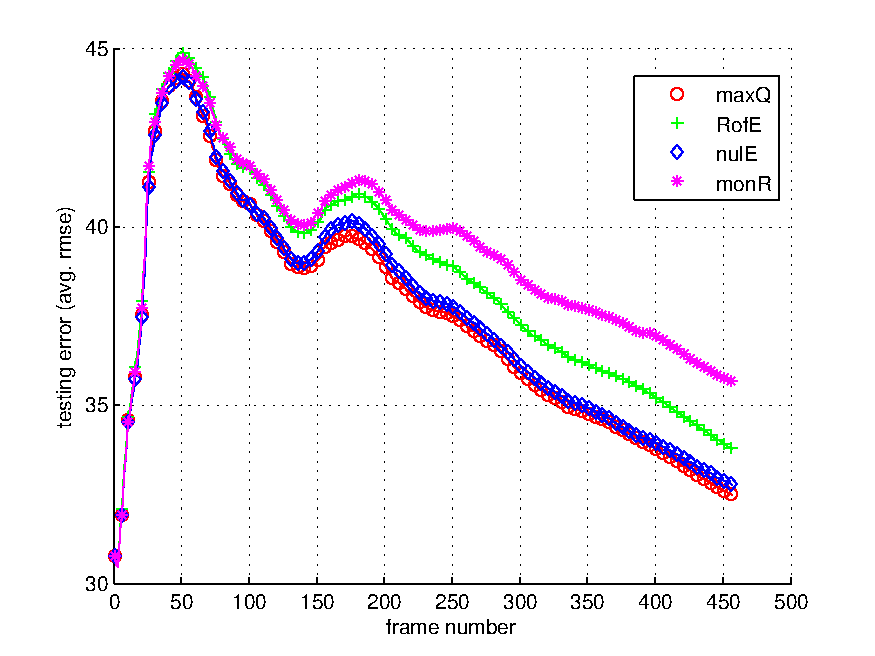
\includegraphics[height=0.4\textheight]{figs/2_davidin300_8_4_1000_tst_armse.pdf}
								\caption{8x4 RVQ, testing error (avg. rmse).}
								\label{fig:2_davidin300_8_4_1000_tst_armse}
								\end{figure}

								\begin{figure}[h!]
								\centering
								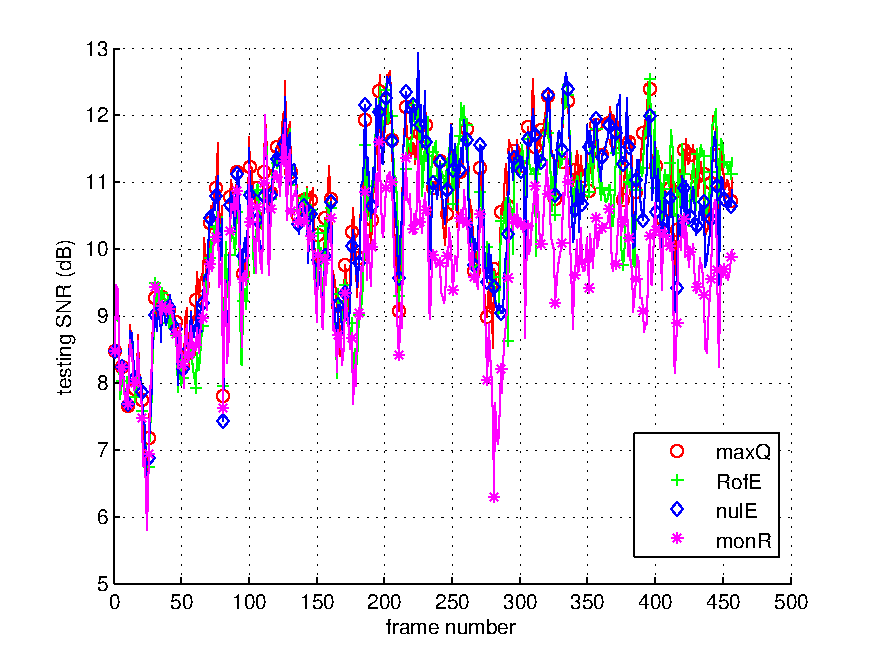
\includegraphics[height=0.4\textheight]{figs/2_davidin300_8_4_1000_tst_SNRdB.pdf}
								\caption{8x4 RVQ,testing SNR in dB.}
								\label{fig:2_davidin300_8_4_1000_tst_SNRdB}
								\end{figure}
